\documentclass{../notes}

\title{决策理论 HW05}

\begin{document}
    \maketitle

    \subparagraph*{1}

    \begin{subquestions}
        \item Jack的决策树如图\ref{fig:dt-1}所示。Jack选择New York会获得$3000$的确定收益,选择Charlotte会获得$50\% \times 5000 + 50\%\times 2500 = 3750$的期望收益,因此Jack应当选择Charlotte。

        \begin{figure}[h]
            \centering
            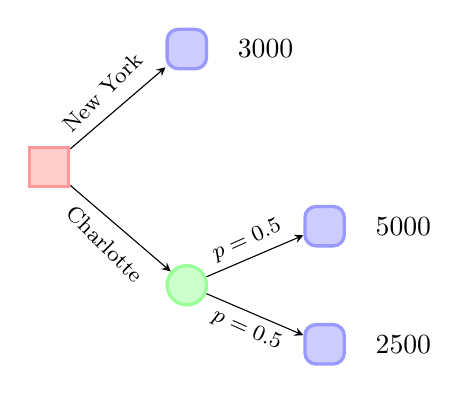
\begin{tikzpicture}
                [
                    DecisionNode/.style={rectangle, draw=red!40, fill=red!20, very thick, minimum size = 5mm},
                    ChanceNode/.style={circle, draw=green!40, fill=green!20, very thick, minimum size = 5mm},
                    ResultNode/.style={rectangle, rounded corners, draw=blue!40, fill=blue!20, very thick, minimum size = 5mm},
                    Connection/.style={-stealth},
                    Label/.style={font=\footnotesize}
                ]
                \node[DecisionNode](Root){};
                \node[ResultNode, right of=Root, xshift=0.75cm, yshift=1.5cm](NewYork){};
                \node[ChanceNode, right of=Root, xshift=0.75cm, yshift=-1.5cm](Charlotte){};
                \node[ResultNode, right of=Charlotte, xshift=0.75cm, yshift=0.75cm](Charlotte-Win){};
                \node[ResultNode, right of=Charlotte, xshift=0.75cm, yshift=-0.75cm](Charlotte-Lose){};

                \draw[Connection] (Root) -> node[Label, xshift=-0.2cm, yshift=0.2cm, rotate=45] {New York} (NewYork);
                \draw[Connection] (Root) -> node[Label, xshift=-0.2cm, yshift=-0.2cm, rotate=-45] {Charlotte} (Charlotte);
                \draw[Connection] (Charlotte) -> node[Label, xshift=-0.1cm, yshift=0.2cm, rotate=24] {$p=0.5$} (Charlotte-Win);
                \draw[Connection] (Charlotte) -> node[Label, xshift=-0.1cm, yshift=-0.2cm, rotate=-24] {$p=0.5$} (Charlotte-Lose);

                \node[right of=NewYork]{$3000$};
                \node[right of=Charlotte-Win]{$5000$};
                \node[right of=Charlotte-Lose]{$2500$};
            \end{tikzpicture}
            \caption{决策树}
            \label{fig:dt-1}
        \end{figure}

        计算可得

        \begin{table}[ht]
            \centering
            \caption{不同结果条件下的Return Load概率}
            \begin{tabular}{ccc}
                \toprule
                预测情况 & RL & NL \\
                \midrule
                B & $\frac{9}{11}$ & $\frac{2}{11}$ \\
                S & $\frac{1}{9}$ & $\frac{8}{9}$ \\
                \bottomrule
            \end{tabular}
        \end{table}

        当咨询结果为B时,前往Charlotte的期望收益为$\frac{9}{11} \times 5000 + \frac{2}{11}\times 2500 = \frac{50000}{11} > 3000$,当咨询结果为$S$时,前往Charlotte的期望收益为$\frac{1}{9} \times 5000 + \frac{8}{9}\times 2500 = \frac{25000}{9} < 3000$。因此应当在咨询结果为B时前往Charlotte,在咨询结果为S时前往New York。

        \item 当最终结果为RL时,咨询的期望收益为

        \begin{equation}
            3000\times 0.45 + \frac{50000}{11} \times 0.55 = 3850
        \end{equation}

        当最终结果为NL时,咨询的期望收益为

        \begin{equation}
            3000\times 0.55 + \frac{25000}{9} \times 0.45 = 2900
        \end{equation}

        因此额外信息的价值为$3850 - 3750 = 100$
    \end{subquestions}

    \subparagraph*{2}

    \begin{subquestions}
        \item 当使用贝叶斯决策准则时,有

        \begin{equation}
            \begin{aligned}
                r(\pi, d_1) &= 0.6\times (-50000) + 0.4\times (-30000) \\
                &= -42000 \\
                r(\pi, d_2) &= 0.6\times (-100000) + 0.4\times 40000 \\
                &= -44000 \\
                r(\pi, d_3) &= 0.6\times (-30000) + 0.4\times (-10000) \\
                &= -22000 \\
            \end{aligned}
        \end{equation}

        决策者会选择$d_2$,即投资办公楼。根据MinMax准则,决策者会选择$d_1$,即投资公寓楼。

        \item 当最终经济状况为G时,有$P(P|G) = \frac{12}{13}, P(N|G) = \frac{1}{13}$,则:

        \begin{equation}
            \begin{aligned}
                r(\pi, d_1) &= \frac{12}{13}\times (-50000) + \frac{1}{13}\times (-30000) \\
                &= -\frac{630000}{13} \\
                r(\pi, d_2) &= \frac{12}{13}\times (-100000) + \frac{1}{13}\times 40000 \\
                &= -\frac{1160000}{13} \\
                r(\pi, d_3) &= \frac{12}{13}\times (-30000) + \frac{1}{13}\times (-10000) \\
                &= -\frac{370000}{13} \\
            \end{aligned}
        \end{equation}

        此时会选择投资办公楼。

        当最终经济状况为P时,有$P(P|P) = \frac{1}{4}, P(N|P) = \frac{3}{4}$,则:

        \begin{equation}
            \begin{aligned}
                r(\pi, d_1) &= \frac{1}{4}\times (-50000) + \frac{3}{4}\times (-30000) \\
                &= -\frac{140000}{4} \\
                r(\pi, d_2) &= \frac{1}{4}\times (-100000) + \frac{3}{4}\times 40000 \\
                &= \frac{20000}{4} \\
                r(\pi, d_3) &= \frac{1}{4}\times (-30000) + \frac{3}{4}\times (-10000) \\
                &= -\frac{-60000}{13} \\
            \end{aligned}
        \end{equation}

        此时会选择投资公寓楼。

        \item 当预测结果为P时,

        \begin{equation}
            -35000\times 0.48 - \frac{1160000}{13} \times 0.52 = -63200
        \end{equation}

        因此信息的价值为$63200 - 44000=19200$
    \end{subquestions}

\end{document}